\documentclass[aspectratio=169, 12pt]{beamer}
\usepackage{fontspec}
\setmainfont{Arial}

\usetheme{Madrid}
\usecolortheme{default}

\usepackage{graphicx}
\usepackage{amsmath}
\usepackage{listings}
\usepackage{booktabs}
\usepackage{xcolor}
\usepackage{tabularx}
\usepackage{caption}

% Set code listing style
\lstset{
    basicstyle=\ttfamily\small,
    breaklines=true,
    keywordstyle=\color{blue},
    stringstyle=\color{red},
    commentstyle=\color{green!60!black},
    showstringspaces=false,
    frame=single,
    backgroundcolor=\color{gray!10}
}

\title[ML - Chap 16]{Chương 16: Xử lý Ngôn ngữ Tự nhiên với RNN và Cơ chế Chú ý}
\author[Giảng viên]{Giảng viên}
\institute[Đại học Đông Á]{Đại học Đông Á}
\date{\today}

\begin{document}

\begin{frame}
    \titlepage
\end{frame}

\begin{frame}{Mục tiêu của Chương}
    \begin{itemize}
        \item Hiểu rõ và áp dụng RNN để xây dựng mô hình sinh văn bản tự động.
        \item Thực hành bài toán Phân tích cảm xúc (Sentiment Analysis) sử dụng Keras.
        \item Nắm vững kiến trúc mạng Encoder-Decoder dùng trong Dịch máy thần kinh (NMT).
        \item Phân tích chi tiết Cơ chế Chú ý (Attention Mechanisms) để khắc phục nhược điểm cổ chai của RNN.
        \item Tiếp cận và sử dụng siêu kiến trúc Transformer (BERT, GPT, ViT) thông qua thư viện Hugging Face.
    \end{itemize}
\end{frame}

\begin{frame}{Mục lục}
    \tableofcontents
\end{frame}

%==================================================================
\section{1. Tạo văn bản kiểu Shakespeare bằng cách sử dụng RNN ký tự}
%==================================================================

\begin{frame}{1.1 Giới thiệu bài toán mô hình hóa ngôn ngữ (Language Modeling)}
    \begin{itemize}
        \item \textbf{Khái niệm:} Mô hình hóa ngôn ngữ là nhiệm vụ dự đoán ký tự (hoặc từ) tiếp theo trong một chuỗi, dựa trên các ký tự (hoặc từ) trước đó.
        \item \textbf{Ứng dụng thực tế:}
            \begin{itemize}
                \item Gợi ý từ khi gõ phím (Autosuggest).
                \item Sửa lỗi chính tả tự động (Spell checking).
                \item Sinh văn bản sáng tạo (Viết thơ, viết truyện, sinh code).
            \end{itemize}
        \item \textbf{Vai trò của RNN:} Một mô hình RNN có khả năng duy trì trạng thái ẩn (hidden state) giúp "ghi nhớ" ngữ cảnh từ quá khứ, rất phù hợp cho dữ liệu văn bản tuần tự.
    \end{itemize}
\end{frame}

\begin{frame}{1.2 Mô hình hóa Cấp độ Ký tự (Character-level) vs Từ (Word-level)}
    \begin{columns}
        \begin{column}{0.5\textwidth}
            \textbf{Mô hình Character-level}
            \begin{itemize}
                \item Dự đoán từng chữ cái một.
                \item Từ vựng nhỏ (vài chục ký tự).
                \item Xử lý tốt từ mới (Out-Of-Vocabulary) và lỗi chính tả.
                \item \textbf{Nhược điểm}: Chuỗi vào quá dài, mô hình dễ quên ngữ cảnh xa.
            \end{itemize}
        \end{column}
        \begin{column}{0.5\textwidth}
            \textbf{Mô hình Word-level}
            \begin{itemize}
                \item Dự đoán từng từ một.
                \item Từ vựng rất lớn (hàng chục, hàng trăm ngàn từ).
                \item Nắm bắt ngữ nghĩa tốt hơn, chuỗi ngắn hơn.
                \item \textbf{Nhược điểm}: Khó xử lý từ hiếm gặp, kích thước ma trận Embedding khổng lồ.
            \end{itemize}
        \end{column}
    \end{columns}
\end{frame}

\begin{frame}{1.3 Tập dữ liệu văn bản Shakespeare}
    \begin{itemize}
        \item Trong ví dụ này, ta sử dụng toàn bộ tác phẩm của Shakespeare làm tập huấn luyện.
        \item Dữ liệu bao gồm các vở kịch, thơ, được gộp chung thành một file văn bản.
        \item Ta tải dữ liệu văn bản bằng Keras: \texttt{keras.utils.get\_file()}.
        \item Văn bản chứa hơn 1 triệu ký tự, bao gồm các chữ cái (viết hoa/viết thường), dấu câu và khoảng trắng.
    \end{itemize}
\end{frame}

\begin{frame}[fragile]{1.4 Tiền xử lý văn bản: Tokenizer trong Keras}
    \begin{itemize}
        \item Mô hình nơ-ron không hiểu chữ cái, nó chỉ hiểu con số.
        \item Ta cần chuyển các ký tự thành số nguyên (ID) bằng Tokenizer.
        \item Keras hỗ trợ lớp \texttt{Tokenizer} cấu hình ở cấp độ ký tự.
    \end{itemize}
\begin{lstlisting}[language=Python]
from tensorflow import keras
# Khoi tao Tokenizer cap do ky tu
tokenizer = keras.preprocessing.text.Tokenizer(char_level=True)
tokenizer.fit_on_texts(shakespeare_text)
# Chuoi "First" -> [20, 6, 9, 8, 3]
max_id = len(tokenizer.word_index) # Tong so ky tu duy nhat (~39)
dataset_size = tokenizer.document_count # Tong ky tu (> 1 trieu)
\end{lstlisting}
\end{frame}

\begin{frame}{1.5 Chuẩn bị dữ liệu bằng tf.data}
    \begin{columns}
        \begin{column}{0.5\textwidth}
            \begin{itemize}
                \item Ta tạo một cửa sổ (window) trượt qua văn bản để tạo ra các cặp (đầu vào, mục tiêu).
                \item Nếu chuỗi là "Thanh", window kích thước 4.
                \item Input: "Tha", Target: "h".
                \item Để tăng tốc, ta dùng \texttt{window(shift=1)} và \texttt{batch} dữ liệu.
            \end{itemize}
        \end{column}
        \begin{column}{0.5\textwidth}
            \centering
            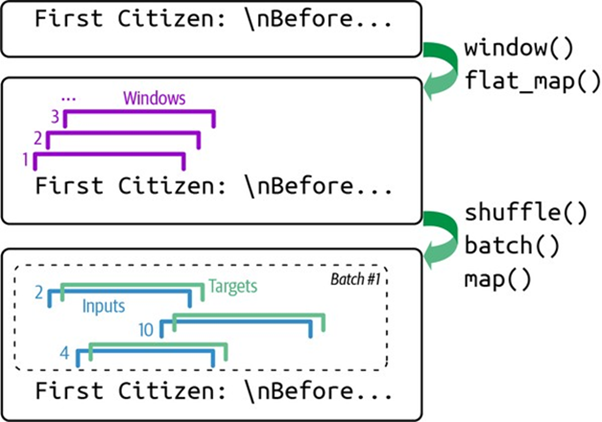
\includegraphics[width=\textwidth,height=0.6\textheight,keepaspectratio]{../machineLearningWeb/Figures/CH16/Hình_16-1.png}
            \vspace{0.2cm}
            \textit{Hình 16-1: Tóm tắt các bước chuẩn bị tập dữ liệu}
        \end{column}
    \end{columns}
\end{frame}

\begin{frame}{1.6 One-hot Encoding so với Embedding}
    \begin{itemize}
        \item \textbf{One-hot Encoding:} Biến số 5 thành véc-tơ $[0, 0, 0, 0, 1, 0, \dots]$.
            \begin{itemize}
                \item Phù hợp khi bộ từ vựng rất nhỏ (39 ký tự).
                \item Không mang thông tin ngữ nghĩa.
            \end{itemize}
        \item \textbf{Embedding:} Biến số 5 thành véc-tơ số thực liên tục $[0.12, -0.5, 0.8, \dots]$.
            \begin{itemize}
                \item Mô hình học được các biểu diễn ẩn tốt hơn.
                \item Thường là lựa chọn tối ưu cho cả Word-level và Character-level hiện nay.
            \end{itemize}
    \end{itemize}
\end{frame}

\begin{frame}[fragile]{1.7 Xây dựng mô hình Char-RNN với GRU}
    \begin{itemize}
        \item Mô hình Char-RNN gồm một lớp Embedding, các lớp GRU (hoặc LSTM) và một lớp Dense phân loại.
        \item \texttt{return\_sequences=True} đảm bảo mỗi bước thời gian của lớp GRU trước đều đẩy kết quả lên lớp GRU sau.
    \end{itemize}
\begin{lstlisting}[language=Python]
model = keras.models.Sequential([
    keras.layers.Embedding(input_dim=num_chars, output_dim=16, 
                           input_length=max_id),
    keras.layers.GRU(128, return_sequences=True, dropout=0.2),
    keras.layers.GRU(128, return_sequences=True, dropout=0.2),
    keras.layers.TimeDistributed(keras.layers.Dense(num_chars, 
                                 activation="softmax"))
])
\end{lstlisting}
\end{frame}

\begin{frame}{1.8 Vấn đề Lặp văn bản khi Dự đoán (Argmax Loop)}
    \begin{itemize}
        \item Nếu tại mỗi bước sinh ký tự mới, ta luôn chọn ký tự có xác suất cao nhất (\textbf{argmax}), văn bản tạo ra sẽ rất nhạt nhẽo.
        \item Nguy hiểm hơn, mô hình có thể bị mắc kẹt trong vòng lặp vô tận (vd: "To be or not to be or not to be...").
        \item \textbf{Lý do:} Mô hình có xu hướng lặp lại các cụm từ phổ biến nhất và an toàn nhất trong tập dữ liệu.
        \item \textbf{Giải pháp:} Sử dụng việc \textbf{lấy mẫu ngẫu nhiên (Sampling)} dựa trên phân bố xác suất thay vì argmax.
    \end{itemize}
\end{frame}

\begin{frame}[fragile]{1.9 Sinh văn bản với Nhiệt độ (Temperature)}
    \begin{itemize}
        \item Thay vì lấy logit trực tiếp, ta chia logit cho tham số \textbf{Temperature} ($T$) trước khi tính Softmax.
        \item $T \approx 0.1$: Chọn ký tự an toàn, chuẩn xác (giống argmax).
        \item $T \approx 1.0$: Lấy mẫu ngẫu nhiên bình thường.
        \item $T \approx 2.0$: Làm phẳng phân bố, tăng tính sáng tạo nhưng dễ sinh ra từ vô nghĩa.
    \end{itemize}
\begin{lstlisting}[language=Python]
import tensorflow as tf
# logits la mang xac suat tu mo hinh
rescaled_logits = logits / temperature
char_id = tf.random.categorical(rescaled_logits, num_samples=1)
\end{lstlisting}
\end{frame}

%==================================================================
\section{2. Phân tích cảm xúc (Sentiment Analysis)}
%==================================================================

\begin{frame}{2.1 Giới thiệu bài toán phân tích cảm xúc}
    \begin{columns}
        \begin{column}{0.5\textwidth}
            \begin{itemize}
                \item \textbf{Nhiệm vụ:} Phân loại văn bản thành cảm xúc "tích cực" (1) hoặc "tiêu cực" (0).
                \item \textbf{Tập dữ liệu:} \textbf{IMDb Reviews} chứa 50.000 bài đánh giá phim.
                \item \textbf{Thách thức}: Làm sao xử lý số lượng từ vựng khổng lồ (hàng chục ngàn từ) và biến chúng thành mảng số để đưa vào mạng?
            \end{itemize}
        \end{column}
        \begin{column}{0.5\textwidth}
            \centering
            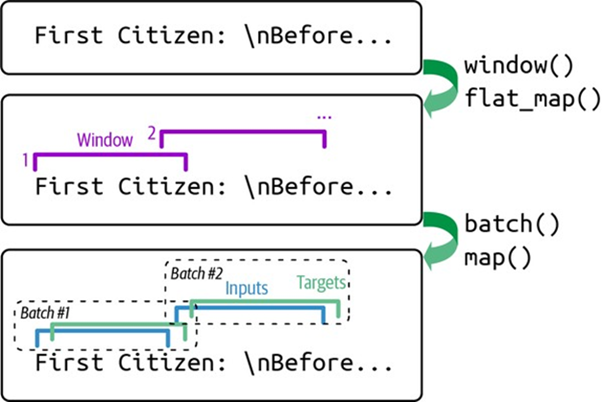
\includegraphics[width=\textwidth,height=0.6\textheight,keepaspectratio]{../machineLearningWeb/Figures/CH16/Hình_16-2.png}
            \vspace{0.2cm}
            \textit{Hình 16-2: Tóm tắt các bước xử lý dữ liệu IMDb}
        \end{column}
    \end{columns}
\end{frame}

\begin{frame}{2.2 Xử lý dữ liệu ngôn ngữ (Word-level)}
    \begin{itemize}
        \item \textbf{Tokenization}: Cắt câu thành các từ (tokens). Loại bỏ dấu câu và HTML tags (như \texttt{<br/>}).
        \item \textbf{Xây dựng từ điển (Vocabulary)}: Ánh xạ mỗi từ thành một số ID nguyên (ví dụ: "the" -> 1, "movie" -> 2).
        \item \textbf{Cắt bớt từ vựng (Truncation)}: Chỉ giữ lại 10.000 từ phổ biến nhất để giảm tải bộ nhớ và tính toán.
        \item Các từ hiếm (Out-Of-Vocabulary) sẽ được gán chung một ID đặc biệt là \texttt{<OOV>}.
    \end{itemize}
\end{frame}

\begin{frame}[fragile]{2.3 Padding và Masking trong Keras}
    \begin{itemize}
        \item \textbf{Padding}: Các bài đánh giá có độ dài khác nhau. Ta cần đệm thêm số 0 ở cuối (hoặc đầu) để đưa về cùng một độ dài max (vd: 500 từ).
        \item \textbf{Masking (\texttt{mask\_zero=True})}: Mạng RNN phải tính toán theo thời gian. Nếu chuỗi có hàng trăm số 0 đệm, RNN sẽ học sai lệch. Việc bật Masking giúp Keras tự động bỏ qua các giá trị đệm 0 này.
    \end{itemize}
\begin{lstlisting}[language=Python]
keras.layers.Embedding(vocab_size, embed_size, 
                       input_shape=[None], mask_zero=True)
\end{lstlisting}
\end{frame}

\begin{frame}[fragile]{2.4 Kiến trúc LSTM cho Phân tích Cảm xúc}
    \begin{itemize}
        \item Sử dụng \texttt{Embedding} để học biểu diễn từ liên tục.
        \item 2 lớp \texttt{GRU} (Gated Recurrent Unit) xếp chồng lên nhau giúp trích xuất ngữ cảnh dài hạn (ai làm gì, sắc thái chê hay khen).
        \item Lớp \texttt{Dense} cuối dùng \texttt{sigmoid} để ra xác suất 0-1.
    \end{itemize}
\begin{lstlisting}[language=Python]
model = keras.models.Sequential([
    keras.layers.Embedding(vocab_size, embed_size, mask_zero=True),
    keras.layers.GRU(128, return_sequences=True),
    keras.layers.GRU(128),
    keras.layers.Dense(1, activation="sigmoid")
])
\end{lstlisting}
\end{frame}

\begin{frame}{2.5 Đánh giá Kết quả và Hạn chế}
    \begin{itemize}
        \item Với RNN/GRU/LSTM, độ chính xác trên tập IMDb có thể dễ dàng đạt \textbf{85\% - 90\%}.
        \item \textbf{Hạn chế 1 (Ngữ nghĩa):} Khó phân tích những bình luận có cấu trúc đảo ngữ phức tạp, dùng từ lóng, hoặc những câu mang tính mỉa mai (Sarcasm).
        \item \textbf{Hạn chế 2 (Tốc độ):} Mô hình có thể bị chậm do chuỗi dài (500 từ) và kiến trúc RNN không thể thực hiện tính toán song song.
    \end{itemize}
\end{frame}

%==================================================================
\section{3. Mạng mã hóa-giải mã cho dịch máy thần kinh}
%==================================================================

\begin{frame}{3.1 Dịch máy thần kinh (Neural Machine Translation - NMT)}
    \begin{columns}
        \begin{column}{0.55\textwidth}
            \begin{itemize}
                \item Kiến trúc \textbf{Encoder-Decoder} là chuẩn mực cho các bài toán sequence-to-sequence (seq2seq).
                \item \textbf{Bộ mã hóa (Encoder)}: Đọc toàn bộ câu nguồn (ví dụ: tiếng Anh) và nén thành một véc-tơ trạng thái (Context Vector).
                \item \textbf{Bộ giải mã (Decoder)}: Nhận Context Vector làm điểm khởi đầu để sinh ra câu đích (ví dụ: tiếng Việt).
            \end{itemize}
        \end{column}
        \begin{column}{0.45\textwidth}
            \centering
            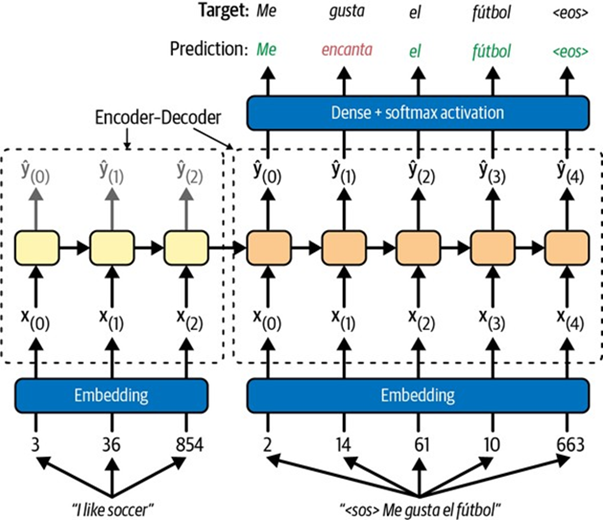
\includegraphics[width=\textwidth,height=0.6\textheight,keepaspectratio]{../machineLearningWeb/Figures/CH16/Hình_16-3.png}
            \vspace{0.2cm}
            \textit{Hình 16-3: Mô hình Encoder-Decoder cơ bản}
        \end{column}
    \end{columns}
\end{frame}

\begin{frame}{3.2 Cơ chế hoạt động của Decoder}
    \begin{columns}
        \begin{column}{0.5\textwidth}
            \begin{itemize}
                \item Tại thời điểm $t$, Decoder lấy từ đã dự đoán ở bước $t-1$ làm đầu vào cho bước tiếp theo.
                \item Nhưng trong khi huấn luyện, để tránh sai lầm dây chuyền, ta dùng \textbf{Teacher Forcing}: cung cấp từ mục tiêu thực tế (ground truth) làm đầu vào.
                \item Token \texttt{<sos>} báo hiệu bắt đầu dịch, và \texttt{<eos>} báo hiệu câu hoàn thành.
            \end{itemize}
        \end{column}
        \begin{column}{0.5\textwidth}
            \centering
            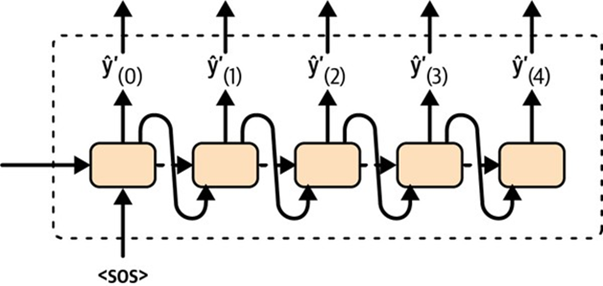
\includegraphics[width=\textwidth,height=0.6\textheight,keepaspectratio]{../machineLearningWeb/Figures/CH16/Hình_16-4.png}
            \vspace{0.2cm}
            \textit{Hình 16-4: Chi tiết cấu trúc Encoder-Decoder}
        \end{column}
    \end{columns}
\end{frame}

\begin{frame}{3.3 Kiến trúc Encoder-Decoder Thực tế (Xếp chồng)}
    \begin{columns}
        \begin{column}{0.4\textwidth}
            \begin{itemize}
                \item Một mạng dịch thuật mạnh mẽ thường dùng nhiều lớp RNN/LSTM xếp chồng (VD: 2 đến 8 lớp).
                \item Trạng thái ẩn cuối cùng của toàn bộ các lớp trong Encoder sẽ được gán làm trạng thái ẩn khởi tạo cho các lớp tương ứng của Decoder.
            \end{itemize}
        \end{column}
        \begin{column}{0.6\textwidth}
            \centering
            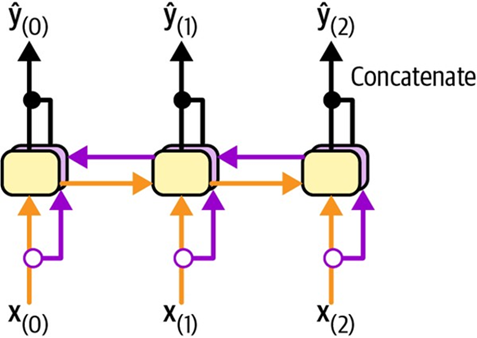
\includegraphics[width=\textwidth,height=0.6\textheight,keepaspectratio]{../machineLearningWeb/Figures/CH16/Hình_16-5.png}
            \vspace{0.2cm}
            \textit{Hình 16-5: Kiến trúc mạng NMT chi tiết với nhiều lớp LSTM}
        \end{column}
    \end{columns}
\end{frame}

\begin{frame}{3.4 Kỹ thuật Tìm kiếm chùm (Beam Search)}
    \begin{columns}
        \begin{column}{0.5\textwidth}
            \begin{itemize}
                \item Nếu chỉ chọn từ có xác suất cao nhất ở mỗi bước (Greedy Search), nếu từ đầu tiên bị sai, toàn bộ câu sau sẽ hỏng.
                \item \textbf{Beam Search} khắc phục bằng cách theo dõi $k$ chuỗi ứng viên (beam width) hứa hẹn nhất cùng lúc.
                \item Tại mỗi bước, nó mở rộng $k$ chuỗi này và giữ lại top $k$ chuỗi có xác suất tích lũy cao nhất để đi tiếp.
            \end{itemize}
        \end{column}
        \begin{column}{0.5\textwidth}
            \centering
            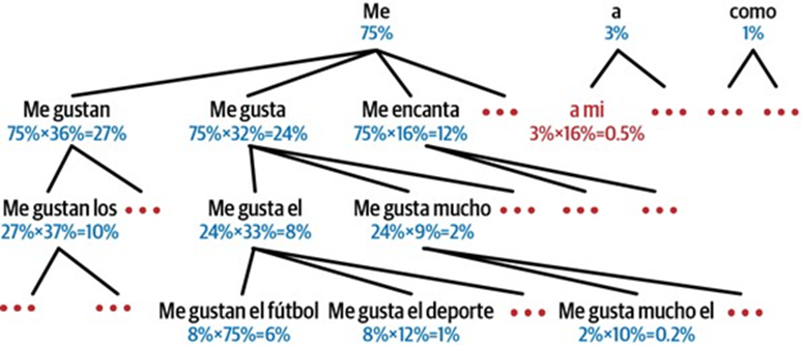
\includegraphics[width=\textwidth,height=0.65\textheight,keepaspectratio]{../machineLearningWeb/Figures/CH16/Hình_16-6.png}
            \vspace{0.2cm}
            \textit{Hình 16-6: Minh họa Beam Search với k=3}
        \end{column}
    \end{columns}
\end{frame}

\begin{frame}{3.5 Đo lường độ tốt của Dịch máy (BLEU Score)}
    \begin{itemize}
        \item Khác với phân loại văn bản, dịch máy không có độ chính xác (Accuracy) tuyệt đối vì một câu có thể được dịch theo nhiều cách đúng đắn.
        \item Thang đo chuẩn mực: \textbf{BLEU (Bilingual Evaluation Understudy)}.
        \item \textbf{Nguyên lý:} Đếm số lượng n-gram (từ hoặc cụm từ) xuất hiện trong bản dịch của máy có khớp với bản dịch tham chiếu của con người hay không.
        \item \textbf{Hình phạt (Penalty):} Trừ điểm nếu mô hình cố tình dịch câu quá ngắn để ăn gian xác suất khớp.
    \end{itemize}
\end{frame}

%==================================================================
\section{4. Cơ chế chú ý (Attention Mechanisms)}
%==================================================================

\begin{frame}{4.1 Vấn đề Nút thắt cổ chai (Bottleneck) của RNN}
    \begin{itemize}
        \item Mô hình Encoder-Decoder truyền thống ép toàn bộ câu nguồn, dù dài hay ngắn, vào một \textbf{véc-tơ trạng thái tĩnh có kích thước cố định} (Context Vector).
        \item Khi câu nguồn rất dài (ví dụ: 50 từ), véc-tơ nhỏ bé này không đủ sức chứa mọi thông tin. Kết quả là mô hình thường "quên" phần đầu câu.
        \item Đây chính là hiện tượng nút thắt cổ chai thông tin.
    \end{itemize}
\end{frame}

\begin{frame}{4.2 Cơ chế Chú ý của Bahdanau (2014)}
    \begin{columns}
        \begin{column}{0.4\textwidth}
            \begin{itemize}
                \item \textbf{Giải pháp:} Thay vì bắt Decoder phải nhớ tất cả từ đầu, cho phép nó "nhìn lại" toàn bộ câu nguồn tại \textbf{mỗi bước dịch}.
                \item Tính toán \textbf{Trọng số chú ý}: Từ đích hiện tại có liên quan chặt chẽ đến từ nguồn nào nhất?
                \item Tạo ra Context Vector linh hoạt cho từng bước.
            \end{itemize}
        \end{column}
        \begin{column}{0.6\textwidth}
            \centering
            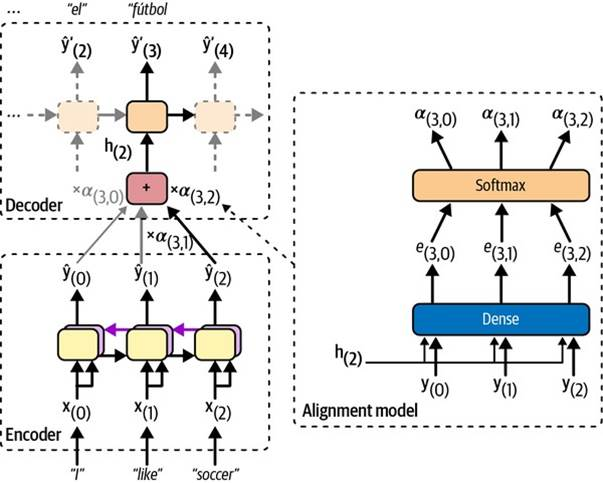
\includegraphics[width=\textwidth,height=0.7\textheight,keepaspectratio]{../machineLearningWeb/Figures/CH16/Hình_16-7.jpg}
            \vspace{0.2cm}
            \textit{Hình 16-7: Encoder-Decoder với Cơ chế Chú ý}
        \end{column}
    \end{columns}
\end{frame}

\begin{frame}{4.3 Sự Ra Đời Của Cú sốc "Transformer" (2017)}
    \begin{itemize}
        \item Bài báo huyền thoại: \textbf{"Attention Is All You Need"} (Vaswani et al., Google, 2017).
        \item \textbf{Tuyên bố chấn động:} "Chúng tôi loại bỏ hoàn toàn cấu trúc RNN tuần tự. Chỉ sử dụng Attention thuần túy!"
        \item \textbf{Vì sao loại bỏ RNN?}
            \begin{itemize}
                \item RNN xử lý tuần tự từng từ $\rightarrow$ Không thể song song hóa $\rightarrow$ Quá chậm trên GPU.
                \item RNN vẫn bị giới hạn khi liên kết thông tin giữa từ thứ 1 và từ thứ 1000. Transformer liên kết chúng trực tiếp bằng độ phức tạp $O(1)$.
            \end{itemize}
    \end{itemize}
\end{frame}

\begin{frame}{4.4 Kiến trúc Transformer Gốc}
    \begin{columns}
        \begin{column}{0.4\textwidth}
            \begin{itemize}
                \item Giữ lại ý tưởng Encoder-Decoder.
                \item Bên trong là hàng loạt khối \textbf{Multi-Head Attention} và mạng lan truyền xuôi (Feed Forward).
                \item Bổ sung thêm Skip Connections và Layer Normalization để chống suy biến gradient.
                \item Tốc độ huấn luyện tăng vọt nhờ GPU.
            \end{itemize}
        \end{column}
        \begin{column}{0.6\textwidth}
            \centering
            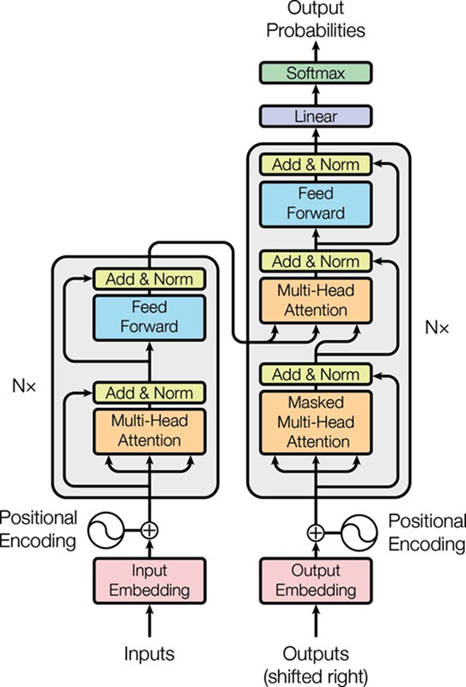
\includegraphics[width=\textwidth,height=0.75\textheight,keepaspectratio]{../machineLearningWeb/Figures/CH16/Hình_16-8.png}
            \vspace{0.1cm}
            \textit{Hình 16-8: Kiến trúc siêu việt của Transformer}
        \end{column}
    \end{columns}
\end{frame}

\begin{frame}{4.5 Mã hóa Vị trí (Positional Encoding)}
    \begin{columns}
        \begin{column}{0.5\textwidth}
            \begin{itemize}
                \item Transformer xử lý tất cả các từ cùng lúc (song song), nên nó mất đi khái niệm về \textbf{thứ tự từ}.
                \item Đối với Transformer, "Chó cắn mèo" và "Mèo cắn chó" là giống hệt nhau nếu không có thứ tự.
                \item \textbf{Giải pháp:} Cộng thêm một véc-tơ tạo bằng hàm Sin/Cosin vào mỗi từ để chỉ định vị trí của nó.
            \end{itemize}
        \end{column}
        \begin{column}{0.5\textwidth}
            \centering
            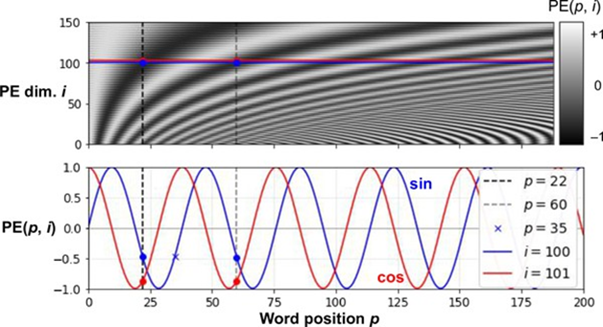
\includegraphics[width=\textwidth,height=0.6\textheight,keepaspectratio]{../machineLearningWeb/Figures/CH16/Hình_16-9.png}
            \vspace{0.2cm}
            \textit{Hình 16-9: Hàm Sine và Cosine trong Positional Encoding}
        \end{column}
    \end{columns}
\end{frame}

\begin{frame}{4.6 Cơ chế Tự Chú ý (Self-Attention)}
    \begin{itemize}
        \item Trong dịch máy trước đây, Decoder chú ý vào Encoder.
        \item \textbf{Self-Attention:} Một câu tự đánh giá mức độ liên quan giữa các từ bên trong chính nó.
        \item Ví dụ: "Ngân hàng (bank) nhà nước nằm bên bờ sông (bank)". Từ "bank" thứ nhất sẽ chú ý nhiều vào "nhà nước", còn "bank" thứ hai chú ý vào "bờ sông". 
        \item Mọi từ đều được cập nhật ý nghĩa dựa trên toàn bộ ngữ cảnh câu.
    \end{itemize}
\end{frame}

\begin{frame}{4.7 Tính toán Q, K, V (Query, Key, Value)}
    \begin{itemize}
        \item Self-Attention được mô hình hóa bằng cơ chế tìm kiếm trong cơ sở dữ liệu:
        \item \textbf{Query (Truy vấn):} Tôi là từ "ngân", tôi đang tìm kiếm cái gì?
        \item \textbf{Key (Khóa):} Tôi là từ "hàng", tôi có chứa thông tin gì?
        \item \textbf{Value (Giá trị):} Ý nghĩa thực sự của tôi là gì.
        \item Transformer dùng phép nhân ma trận giữa Q và K để đo độ tương đồng (Attention Score), sau đó dùng Score này để lấy trọng số cho V.
    \end{itemize}
\end{frame}

\begin{frame}{4.8 Chú ý Đa đầu (Multi-Head Attention)}
    \begin{columns}
        \begin{column}{0.45\textwidth}
            \begin{itemize}
                \item Một cái đầu (Head) không thể hiểu hết sự phức tạp của ngôn ngữ.
                \item \textbf{Multi-Head}: Phân tách phép tính Attention thành $h$ "đầu" khác nhau (vd: 8, 12, hay 96 đầu).
                \item Mỗi đầu sẽ học cách tập trung vào một mối quan hệ riêng (vd: đầu 1 học ngữ pháp, đầu 2 học ý nghĩa, đầu 3 học đại từ nhân xưng).
            \end{itemize}
        \end{column}
        \begin{column}{0.55\textwidth}
            \centering
            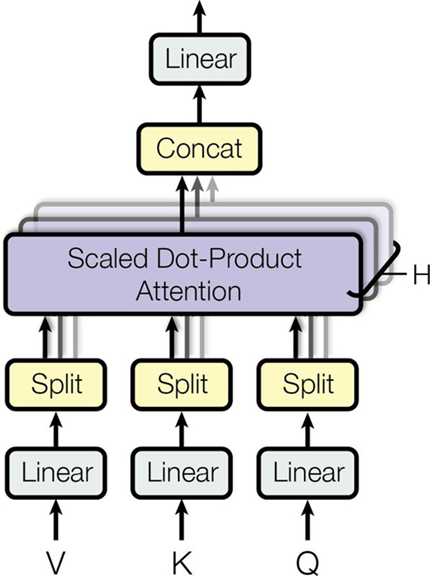
\includegraphics[width=\textwidth,height=0.6\textheight,keepaspectratio]{../machineLearningWeb/Figures/CH16/Hình_16-10.png}
            \vspace{0.2cm}
            \textit{Hình 16-10: Sơ đồ Scaled Dot-Product và Multi-Head}
        \end{column}
    \end{columns}
\end{frame}

\begin{frame}{4.9 Tổng kết: Tại sao Transformer mạnh đến vậy?}
    \begin{itemize}
        \item \textbf{Cơ chế song song (Parallelization):} Huấn luyện nhanh hơn RNN gấp chục lần trên TPU/GPU.
        \item \textbf{Ngữ cảnh toàn cục $O(1)$:} Một từ cuối văn bản có thể liên kết trực tiếp với từ đầu văn bản mà không bị suy giảm thông tin.
        \item \textbf{Khả năng mở rộng không giới hạn (Scalability):} Càng thêm dữ liệu, càng tăng tham số (từ triệu lên hàng trăm tỷ), mô hình càng thông minh đột biến.
    \end{itemize}
\end{frame}

%==================================================================
\section{5. Tuyết lở các mô hình Transformer \& Hugging Face}
%==================================================================

\begin{frame}{5.1 Các Họ Mô Hình Khổng lồ (Foundation Models)}
    \begin{itemize}
        \item Sự ra đời của Transformer chia nhánh phát triển AI thành 3 họ chính:
        \item \textbf{Encoder-only (Họ BERT):} Hiểu văn bản xuất sắc. (Phân loại, trích xuất thực thể).
        \item \textbf{Decoder-only (Họ GPT):} Sinh văn bản xuất sắc. (Chatbot, tạo code, viết báo).
        \item \textbf{Encoder-Decoder (Họ T5, BART):} Cân bằng cả hai. (Dịch thuật, tóm tắt tự động).
    \end{itemize}
\end{frame}

\begin{frame}{5.2 Kiến trúc BERT (Bi-directional Encoder)}
    \begin{columns}
        \begin{column}{0.5\textwidth}
            \begin{itemize}
                \item \textbf{BERT (Google, 2018)}: Chỉ sử dụng phần Encoder.
                \item Kỹ thuật Masked Language Model: Che ngẫu nhiên 15\% từ và ép mô hình phải điền vào chỗ trống bằng cách nhìn cả trước và sau (2 chiều - Bi-directional).
                \item Ứng dụng mạnh mẽ để tinh chỉnh (Fine-tuning) cho các tác vụ NLP hẹp.
            \end{itemize}
        \end{column}
        \begin{column}{0.5\textwidth}
            \centering
            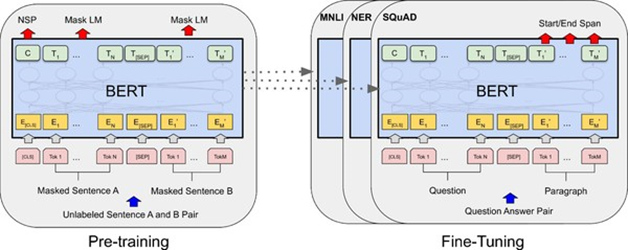
\includegraphics[width=\textwidth,height=0.6\textheight,keepaspectratio]{../machineLearningWeb/Figures/CH16/Hình_16-11.png}
            \vspace{0.2cm}
            \textit{Hình 16-11: Cấu trúc của BERT để huấn luyện đa nhiệm}
        \end{column}
    \end{columns}
\end{frame}

\begin{frame}{5.3 Vision Transformers (ViT) - Attention trong Computer Vision}
    \begin{columns}
        \begin{column}{0.4\textwidth}
            \begin{itemize}
                \item Kỷ nguyên Transformer không chỉ dừng ở NLP.
                \item \textbf{Cách làm:} Cắt ảnh lớn thành lưới các ô nhỏ (patches), chải phẳng và coi mỗi ô như một "từ".
                \item Dùng Transformer phân tích hình ảnh, đạt độ chính xác đánh bại CNN truyền thống (ResNet) trên các tập dữ liệu lớn.
            \end{itemize}
        \end{column}
        \begin{column}{0.6\textwidth}
            \centering
            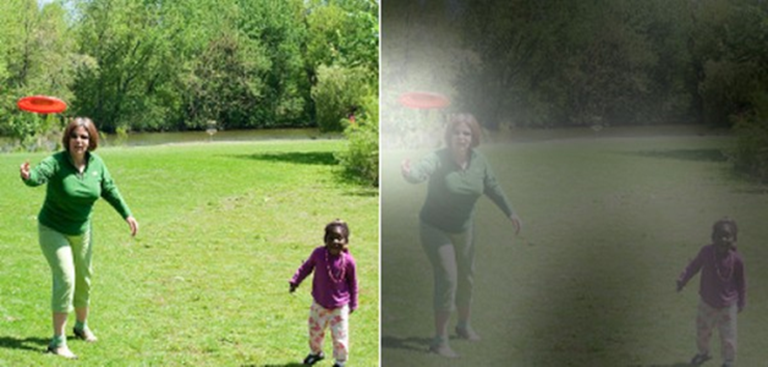
\includegraphics[width=\textwidth,height=0.65\textheight,keepaspectratio]{../machineLearningWeb/Figures/CH16/Hình_16-12.png}
            \vspace{0.2cm}
            \textit{Hình 16-12: Sự tập trung hình ảnh của mô hình Attention}
        \end{column}
    \end{columns}
\end{frame}

\begin{frame}{5.4 Thư viện Transformers của Hugging Face}
    \begin{itemize}
        \item \textbf{Hugging Face} là công ty cung cấp "GitHub cho Machine Learning", sở hữu kho Model Hub lớn nhất thế giới.
        \item Cung cấp các công cụ (Pipeline) mã nguồn mở để tải và sử dụng các mô hình khổng lồ dễ dàng.
        \item Giải phóng lập trình viên khỏi việc phải tự huấn luyện mô hình từ đầu, tiết kiệm hàng triệu đô la tiền thuê máy chủ.
    \end{itemize}
\end{frame}

\begin{frame}[fragile]{5.5 Ví dụ: Tích hợp AI bằng Hugging Face Pipeline}
    \begin{itemize}
        \item Chỉ với 4 dòng code, bạn đã đưa được mô hình State-of-the-Art vào ứng dụng:
    \end{itemize}
\begin{lstlisting}[language=Python]
from transformers import pipeline

# Khoi tao pipeline phan tich cam xuc 
classifier = pipeline("sentiment-analysis")

# Du doan (Tu dong tai mo hinh ve neu chua co)
result = classifier("I really loved this movie, it was fantastic!")
print(result) 
# Ket qua: [{'label': 'POSITIVE', 'score': 0.9998}]
\end{lstlisting}
\end{frame}

\begin{frame}{Tổng Kết Chương 16}
    \begin{itemize}
        \item \textbf{RNN / GRU}: Nền tảng cốt lõi của xử lý dữ liệu tuần tự, nhưng bị giới hạn bởi nút thắt cổ chai và khó song song hóa.
        \item \textbf{Encoder-Decoder}: Kiến trúc vàng cho dịch máy, tạo tiền đề cho các mô hình Seq2seq.
        \item \textbf{Cơ chế Attention}: Cuộc cách mạng giải quyết bài toán bộ nhớ dài hạn, cho phép mô hình nhìn toàn cảnh.
        \item \textbf{Transformer}: Kẻ thay đổi cuộc chơi, khai sinh kỷ nguyên mô hình nền tảng (Foundation Models) và LLM.
        \item \textbf{Hugging Face}: Cầu nối đưa AI tiên tiến đến tay mọi lập trình viên.
    \end{itemize}
\end{frame}

\begin{frame}
    \centering
    \Huge \textbf{HỎI \& ĐÁP}
\end{frame}

\end{document}
